% The rewriting relation \( \Rightarrow_{\mathcal{A},\mathfrak{M}} \) is terminating relative to $\Rightarrow_{\mathcal{B},\mathfrak{M}}$ if the following hold: (i) for all \(G \Rightarrow_{\mathcal{A},\mathfrak{M}} H\), \( w_{s_\mathbb{X}}(G) > w_{s_\mathbb{X}}(H) \), and (ii) for all \(G \Rightarrow_{\mathcal{B},\mathfrak{M}} H\), \( w_{s_\mathbb{X}}(G) \geq w_{s_\mathbb{X}}(H) \). However, directly verifying all rewriting steps is infeasible due to their potential infiniteness. 
% Thus, we aim to provide a rule-based sufficient condition for termination.
% \begin{remark}

\begin{notation}
    % \noindent
    % \begin{minipage}{0.6\textwidth}\setlength{\parindent}{1em}
     Let \( \mathcal{X} = (X, F_X) \) be a ruler-graph. Let \( A, B, G \) be graphs. Let \( \alpha \colon A \to G \) and \( \beta \colon B \to G \) be morphisms. 
    We define the following sets of monomorphisms of $X$ in $G$: 
        %  the set $\operatorname{Mono}(X,G,\alpha)$ of occurrences which is fully included in $A$; the set $\operatorname{Mono}(X,G,\lnot \alpha)$ of occurrences which is not fully included in $A$; the set $\operatorname{Mono}(X,G,\lnot \alpha, \beta)$ of occurrences which is not fully included in $A$ but fully include in $B$; the set $\operatorname{Mono}(X,G,\lnot \alpha, \lnot \beta)$ of occurrences which is neither fully included in $A$ nor fully include in $B$. Formally:
    % \end{minipage}%
    % \begin{minipage}{0.38\textwidth}
    %     \hfill
    %     \begin{tikzpicture}[scale=0.9]
    %         \node (X) at (-0.5,0) {$X$};
    %         \node (G) at (1,0) {$G$}; 
    %         \node (A) at (3,0.2) {$A$}; 
    %         \node (B) at (3,-0.2) {$B$}; 
    %         \draw [>->] (X) to (G);
    %         \draw [>->] (A) to node [above,label,pos=0.5] {$\alpha$} (G);
    %         \draw [>->] (B) to node [below,label,pos=0.5] {$\beta$} (G);
    %     \end{tikzpicture}
    % \end{minipage}%
    \begin{align*}
        \operatorname{Mono}(X,G,\alpha) &= \left\{ \iota \colon X \rightarrowtail G \;\middle|\; \exists \beta \colon X \rightarrowtail A.\, \iota = \beta \star \alpha \right\}, 
        \\
        \operatorname{Mono}(X,G,\lnot \alpha) &= \left\{ \iota \colon X \rightarrowtail G \;\middle|\; \nexists \beta \colon X \rightarrowtail A.\, \iota = \beta \star \alpha \right\}, 
        \\
        \operatorname{Mono}(X,G,\lnot \alpha, \beta) &= \left\{ 
            \iota \colon X \rightarrowtail G \;\middle|\; 
                \begin{aligned}  
                    &(\nexists \zeta \colon X \rightarrowtail A.\, \iota = \zeta \star \alpha) \\ 
                    &\land (\exists \zeta \colon X \rightarrowtail B.\, \iota = \zeta \star \beta)
                \end{aligned}
        \right\},
        \\
        \operatorname{Mono}(X,G,\lnot \alpha, \lnot \beta) &= \left\{ 
            \iota \colon X \rightarrowtail G \;\middle|\; 
                \begin{aligned}
                    &(\nexists \zeta \colon X \rightarrowtail A.\, \iota = \zeta \star \alpha) \\
                    &\land (\nexists \zeta \colon X \rightarrowtail B.\, \iota = \zeta \star \beta)
                \end{aligned}
        \right\}.
    \end{align*}
    For each of the above sets, we introduce the subscript``NF" (respectively ``F") to denote the subset of \( X \)-occurrences that are not included in any \( Y \)-occurrence for all \( Y \in F_X \) (respectively, that are included in some \( Y \)-occurrence for some \( Y \in F_X \)). For example: \( \operatorname{Mono}(X, G, \alpha)_{\text{NF}} \) and \( \operatorname{Mono}(X, G, \alpha)_{\text{F}} \).
\end{notation}
\noindent
\begin{minipage}{0.7\textwidth}\setlength{\parindent}{1em}
    Suppose that all hypothesese in Lemma~\ref{lem:w_u_l_not_geq_r_not} are satisfied. Consider a DPO diagram (illustrated on the right) defining a rewriting step \( G \Rightarrow_{\rho,\mathfrak{M}} H \). 
    The sets of monomorphisms from \( X \) to \( G \) and \( H \) can be decomposed into the following disjoint unions:
\end{minipage}%
\begin{minipage}{0.29\textwidth}
    \hfill
    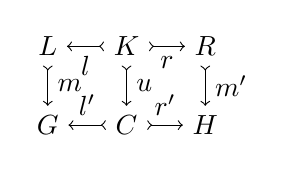
\begin{tikzpicture}
        % [node distance=15mm]
        \node (I) {$K$};
        \node (L) [left of=I] {$L$};
        \node (R) [right of=I] {$R$};
        \node (G) [below of=L] {$G$};
        \node (C) [below of=I] {$C$};
        \node (H) [below of=R] {$H$}; 
        \draw [>->] (I) to  node [midway,below] {$l$} (L);
        \draw [>->] (I) to  node [midway,below] {$r$} (R);
        \draw [>->] (L) to node [midway,right] {$m$} (G);
        \draw [>->] (I) to  node [midway,right] {$u$} (C); 
        \draw [>->] (R) to  node [midway,right] {$m'$} (H);
        \draw [>->] (C) to node [midway,above] {$l'$} (G);
        \draw [>->] (C) to node [midway,above] {$r'$} (H);
        % \node [at=($(I)!.5!(G)$)] {\normalfont PO};
        % \node [at=($(I)!.5!(H)$)] {\normalfont PO};
      \end{tikzpicture}
\end{minipage}

\begin{flalign*}
    \operatorname{Mono}(X,G)_{\operatorname{NF}} &= 
    \operatorname{Mono}(X,G,m)_{\operatorname{NF}}
    \uplus
    \operatorname{Mono}(X,G,\lnot m, l')_{\operatorname{NF}} 
    \uplus
    \operatorname{Mono}(X,G,\lnot m, \lnot l')_{\operatorname{NF}}
    \\
    \operatorname{Mono}(X,H)_{\operatorname{NF}} &= 
    \operatorname{Mono}(X,H,m')_{\operatorname{NF}}
    \uplus
    \operatorname{Mono}(X,H,\lnot m', r')_{\operatorname{NF}}
    \uplus
    \operatorname{Mono}(X,H,\lnot m', \lnot r')_{\operatorname{NF}}
\end{flalign*}
Thus, we have 
\begin{flalign*}
    \card{\operatorname{Mono}(X,G)_{\operatorname{NF}}} - 
    \card{\operatorname{Mono}(X,H)_{\operatorname{NF}}} =& 
    (\operatorname{Mono}(X,G,m)_{\operatorname{NF}} - \operatorname{Mono}(X,H,m')_{\operatorname{NF}}) + \\
    &(\operatorname{Mono}(X,G,\lnot m, l')_{\operatorname{NF}} - \operatorname{Mono}(X,H,\lnot m', r')_{\operatorname{NF}}) + \\
    &(\operatorname{Mono}(X,G,\lnot m, \lnot l')_{\operatorname{NF}} - \operatorname{Mono}(X,H,\lnot m', \lnot r')_{\operatorname{NF}})
\end{flalign*}
We have
$
    \card{\operatorname{Mono}(X,G)_{\operatorname{NF}}} - 
    \card{\operatorname{Mono}(X,H)_{\operatorname{NF}}} \geq 
    \card{\operatorname{Mono}(X,L)} -
    \card{\operatorname{Mono}(X,R)}
$, by the following lemmas under the following assumptions:

\begin{enumerate}[label=(\alph*)]
    \item \label{hyp:inj_mono_x_l_to_r} there exists an injection $M_X$ from $Mono(X,L)_F$ to $Mono(X,R)_F$ such that (todo) for all $h_{XL}$, $h_{XL}$ and $M_X(h_{XL})$ have the same interface elements .
    \item \label{hyp:inj_mono_f_l_to_r} there exists an injection $M_F$ from $Mono(X,L)$ to $Mono(X,R)$ such that (todo)
    \begin{itemize}
        \item for all $h_{XL}$, $h_{XL}$ and $M_X(h_{XL})$ have the same interface elements
        \item for all $h_{XL}:X \rightarrowtail L$, if $h_{XL} = h_{XF} \star h_{FL}$, then $M_X(h_{XL}) = h_{XF} \star M_F(h_{FL})$.
    \end{itemize}  
    \item \label{hyp:f_non_increasing} $\rho^-1$ is $F$-non-increasing.
    \item \label{hyp:f_implicitly_destroyed} for all $L' \in D(L,F)$, let $h_{L'L}:L' \rightarrowtail L$ be the monomorphism give by the $F$-non-increasing property, if there exists $h_{XL'}:X \rightarrowtail L'$ such that $h_{XL} = h_{XL'} \star h_{L'L}$, then $M_X(h_{XL}) = h_{XL'} \star M_L(h_{L'L})$.
    \item $\rho^-1$ and $\rho$ are $X$-non-increasing.
\end{enumerate}.

% \begin{lemma}
%     \label{lem:decomp_w_u}
%     \ \newline
%     \noindent
%     \begin{minipage}{0.7\textwidth}
%         Let $X$ be a ruler-graph. For a pushout square as shown on the right, we have 
%         % $\card{\operatorname{Mono}(X, B)} = \card{\operatorname{Mono}(X, D, \beta')}$ and $\card{\operatorname{Mono}(X, C, \lnot \beta)} = \card{\operatorname{Mono}(X, D, \lnot \beta', \alpha')}$.
%         \begin{flalign*}
%             \card{\operatorname{Mono}(X, B)} &= \card{\operatorname{Mono}(X, D, \beta')}
%             \\
%             \card{\operatorname{Mono}(X, C, \lnot \beta)} &= \card{\operatorname{Mono}(X, D, \lnot \beta', \alpha')}
%         \end{flalign*}
%     \end{minipage}
%     \hfill
%     \begin{minipage}{0.3\textwidth}
%         \hfill
%         \begin{tikzpicture}
%             \node (A) {$A$};
%             \node [below of=A] (B) {$B$}; 
%             \node [left of=A] (C) {$C$}; 
%             \node [left of=B] (D) {$D$}; 
%             \begin{scope}[nodes=rectangle]          
%             \draw [>->] (A) to node [right,label,pos=0.5] {$\alpha$} (B);
%             \draw [>->] (A) to node [above,label,pos=0.5] {$\beta$} (C);
%             \draw [>->] (B) to node [below,label,pos=0.45] {$\beta'$} (D); 
%             \draw [>->] (C) to node [left,label,pos=0.45] {$\alpha'$} (D);
%             \end{scope}
%         \end{tikzpicture}
%     \end{minipage} 
% \end{lemma}
% \begin{proof}
%     See the Appendix,~\autoref{proof:dcomp_w_u}.
%  \end{proof}

\begin{lemma}
    \label{lem:xgm_xhmp_xl_xr}
    % Consider a DPO diagram as shown below 

    % \begin{tikzpicture}
    %     % [node distance=15mm]
    %     \node (I) {$K$};
    %     \node (L) [left of=I] {$L$};
    %     \node (R) [right of=I] {$R$};
    %     \node (G) [below of=L] {$G$};
    %     \node (C) [below of=I] {$C$};
    %     \node (H) [below of=R] {$H$};
    %     \draw [>->] (I) to  node [midway,below] {$l$} (L);
    %     \draw [>->] (I) to  node [midway,below] {$r$} (R);
    %     \draw [>->] (L) to node [midway,right] {$m$} (G);
    %     \draw [>->] (I) to  node [midway,right] {$u$} (C);
    %     \draw [>->] (R) to  node [midway,right] {$m'$} (H);
    %     \draw [>->] (C) to node [midway,above] {$l'$} (G);
    %     \draw [>->] (C) to node [midway,above] {$r'$} (H);
    %     % \node [at=($(I)!.5!(G)$)] {\normalfont PO};
    %     % \node [at=($(I)!.5!(H)$)] {\normalfont PO};
    %   \end{tikzpicture}
    %   we have 
    \begin{flalign*}
        \card{\operatorname{Mono}(X,G,m)_{\operatorname{NF}}} - 
        \card{\operatorname{Mono}(X,H,m')_{\operatorname{NF}}} 
        \geq 
        \card{\operatorname{Mono}(X,L)} -
        \card{\operatorname{Mono}(X,R)}
    \end{flalign*}
\end{lemma}
\begin{proof}
    See the Appendix,~\autoref{proof:lem:xgm_xhmp_xl_xr}.
 \end{proof}


\begin{lemma}
    \label{lem:xglnotmlp_xhlnotmrp}
    % Consider a DPO diagram as shown below 
     
    % \begin{tikzpicture}
    %     % [node distance=15mm]
    %     \node (I) {$K$};
    %     \node (L) [left of=I] {$L$};
    %     \node (R) [right of=I] {$R$};
    %     \node (G) [below of=L] {$G$};
    %     \node (C) [below of=I] {$C$};
    %     \node (H) [below of=R] {$H$};
    %     \draw [>->] (I) to  node [midway,below] {$l$} (L);
    %     \draw [>->] (I) to  node [midway,below] {$r$} (R);
    %     \draw [>->] (L) to node [midway,right] {$m$} (G);
    %     \draw [>->] (I) to  node [midway,right] {$u$} (C);
    %     \draw [>->] (R) to  node [midway,right] {$m'$} (H);
    %     \draw [>->] (C) to node [midway,above] {$l'$} (G);
    %     \draw [>->] (C) to node [midway,above] {$r'$} (H);
    %     % \node [at=($(I)!.5!(G)$)] {\normalfont PO};
    %     % \node [at=($(I)!.5!(H)$)] {\normalfont PO};
    %   \end{tikzpicture}
    
    % We have 
    $
        \card{\operatorname{Mono}(X,G,\lnot m, l')_{\operatorname{NF}}} \geq
        \card{\operatorname{Mono}(X,H,\lnot m', r')_{\operatorname{NF}}}$.
\end{lemma} 
\begin{proof}
    See the Appendix,~\autoref{proof:lem:xglnotmlp_xhlnotmrp}.
 \end{proof}

\begin{lemma}
    \label{lem:xglnotmlnotlp_xhlnotmrnotrp}
    $
        \card{\operatorname{Mono}(X,G,\lnot m, \lnot l')_{\operatorname{NF}}} \geq
        \card{\operatorname{Mono}(X,H,\lnot m', \lnot r')_{\operatorname{NF}}}
    $
\end{lemma}
\begin{proof}
    See the Appendix,~\autoref{proof:lem:xglnotmlnotlp_xhlnotmrnotrp}.
 \end{proof}
Consequently, we have 
\begin{flalign*}
    &w_{s_\mathbb{X}}(G) - w_{s_\mathbb{X}}(H)
    \\
   \overset{\operatorname{def}}{=}&\sum_{X \in \mathbb{X}}^{}s_\mathbb{X}(X) * m_X(G) - \sum_{X \in \mathbb{X}}^{}s_\mathbb{X}(X) * m_X(H)
   \\
   \overset{\operatorname{def}}{=}&\sum_{X \in \mathbb{X}}^{}s_\mathbb{X}(X) * |\operatorname{Mono}(X,G)| - \sum_{X \in \mathbb{X}}^{}s_\mathbb{X}(X) * |\operatorname{Mono}(X,H)|
   \\
   =&\sum_{X \in \mathbb{X}}^{}s_\mathbb{X}(X) * \left( \card{\operatorname{Mono}(X,G)} -  \card{\operatorname{Mono}(X,H)} \right)
   \\
   =&\sum_{X \in \mathbb{X}}^{}s_\mathbb{X}(X) * \card{\operatorname{Mono}(X,G)} -  
   \sum_{X \in \mathbb{X}}^{}s_\mathbb{X}(X) *  \card{\operatorname{Mono}(X,H)}  
    \\
    \overset{\operatorname{def}}{=}&\sum_{X \in \mathbb{X}}^{}s_\mathbb{X}(X) * m_X(L) - \sum_{X \in \mathbb{X}}^{}s_\mathbb{X}(X) * m_X(R)
    \\
    \overset{\operatorname{def}}{=}& w_{s_\mathbb{X}}(L) - w_{s_\mathbb{X}}(R)
\end{flalign*}

The following lemma captures the above reasoning.
\begin{lemma}[Decreasing step]
    \label{lem:w_g_geq_w_h_leq}
    Let $\rho = (L \overset{l}{\leftarrowtail} K \overset{r}{\rightarrowtail} R)$ be an injective DPO rewriting rule,
    \( \mathbb{X} \) a set of ruler-graphs,
    \( s_{\mathbb{X}} \colon \mathbb{X} \to \mathbb{N} \) a weight function,
    and \( G \Rightarrow_{\rho,\mathfrak{M}} H \) a rewriting step. 
    If $\rho$ is \( X \)-non-increasing for every ruler-graph \( X \in \mathbb{X} \), then $
        w_{s_\mathbb{X}}(G) - w_{s_\mathbb{X}}(H) 
        \geq 
        w_{s_\mathbb{X}}(L) - w_{s_\mathbb{X}}(R)
    $.
\end{lemma}
\begin{proof}
    See the Appendix, \hyperref[proof:lem:w_g_geq_w_h_leq]{Section C}.
\end{proof}
Finally, we state our main result.
\begin{theorem}[Termination] 
    \label{thm:termination_grs}
    Let \(\mathcal{A}\) and \(\mathcal{B}\) be sets of injective DPO rewriting rules, $\mathbb{X}$ a set of ruler-graphs and $s_\mathbb{X}$ a weight function. If the following hold:
    \begin{enumerate}
        \item  for every $\rho \in \mathcal{A} \cup \mathcal{B}$ and for every $X \in \mathbb{X}$, the rule $\rho$ is $X$-non-increasing,
        \item for every \(\rho \in \mathcal{A}\), we have \( w_{s_\mathbb{X}}(lhs(\rho)) > w_{s_\mathbb{X}}(rhs(\rho)) \),
        \item for every \(\rho \in \mathcal{B}\), we have \( w_{s_\mathbb{X}}(lhs(\rho)) \geq w_{s_\mathbb{X}}(rhs(\rho)) \).
    \end{enumerate}
    Then \(\Rightarrow_{\mathcal{A},\mathcal{M}}\) is terminating relative to \(\Rightarrow_{\mathcal{B},\mathcal{M}}\).
\end{theorem}
\begin{proof}
    See the Appendix, \hyperref[proof:thm:termination_grs]{Section C}.
\end{proof}